%%
%% ACS project dissertation template.
%%
%% Currently designed for printing two-sided, but if you prefer to
%% print single-sided just remove ",twoside,openright" from the
%% \documentclass[] line below.
%%
%%
%%   SMH, May 2010.


\documentclass[a4paper,12pt,twoside,openright]{report}


%%
%% EDIT THE BELOW TO CUSTOMIZE
%%

\def\authorname{Tom M. Read Cutting\xspace}
\def\authorcollege{Downing College\xspace}
\def\authoremail{tr395@cam.ac.uk}
\def\dissertationtitle{Heterogeneous type checking in multi-language CPU-GPU systems}
\def\wordcount{TODO}


\usepackage{array,color,epsfig,float,inconsolata,graphicx,hyperref,listings,parskip,setspace,tabularx,tabu,xspace}
\graphicspath{ {images/} }

\newfloat{lstfloat}{htbp}{lop}
\floatname{lstfloat}{Listing}
\def\lstfloatautorefname{Listing} % needed for hyperref/auroref

\definecolor{codegreen}{rgb}{0,0.6,0}
\definecolor{codegray}{rgb}{0.5,0.5,0.5}
\definecolor{codepurple}{rgb}{0.58,0,0.82}
\definecolor{backcolour}{rgb}{0.95,0.95,0.92}
\lstdefinestyle{mystyle}{
    backgroundcolor=\color{backcolour},
    commentstyle=\color{codegreen},
    keywordstyle=\color{magenta},
    numberstyle=\tiny\color{codegray},
    stringstyle=\color{codepurple},
    basicstyle=\ttfamily\footnotesize,
    breakatwhitespace=false,
    breaklines=true,
    captionpos=b,
    keepspaces=true,
    numbers=left,
    numbersep=5pt,
    showspaces=false,
    showstringspaces=false,
    showtabs=false,
    tabsize=2
}

\lstset{style=mystyle}

%% START OF DOCUMENT
\begin{document}


%% FRONTMATTER (TITLE PAGE, DECLARATION, ABSTRACT, ETC)
\pagestyle{empty}
\singlespacing
% title page information
\begin{titlepage}

\begin{center}
\noindent
\huge
\dissertationtitle \\
\vspace*{\stretch{1}}
\end{center}

\begin{center}
\noindent
\huge
\authorname \\
\Large
\authorcollege      \\[24pt]

\includegraphics{CUni3.eps}
\end{center}

\vspace{24pt}

\begin{center}
\noindent
\large
{\it A dissertation submitted to the University of Cambridge \\
in partial fulfilment of the requirements for \\
Computer Science Tripos, Part III}
\vspace*{\stretch{1}}
\end{center}

\begin{center}
\noindent
University of Cambridge \\
Department of Computer Science and Technology \\
William Gates Building  \\
15 JJ Thomson Avenue    \\
Cambridge CB3 0FD       \\
{\sc United Kingdom}    \\
\end{center}

\begin{center}
\noindent
Email: \authoremail \\
\end{center}

\begin{center}
\noindent
\today
\end{center}

\end{titlepage}

\newpage
\vspace*{\fill}

\onehalfspacing
\newpage
{\Huge \bf Declaration}

\vspace{24pt}

I \authorname of \authorcollege, being a candidate for the M.Phil in
Advanced Computer Science, hereby declare that this report and the
work described in it are my own work, unaided except as may be
specified below, and that the report does not contain material that
has already been used to any substantial extent for a comparable
purpose.

\vspace{24pt}
Total word count: \wordcount

\vspace{60pt}
\textbf{Signed}:

\vspace{12pt}
\textbf{Date}:


\vfill

This dissertation is copyright \copyright 2018 \authorname.
\\
All trademarks used in this dissertation are hereby acknowledged.



\newpage
\vspace*{\fill}

\singlespacing
\newpage
{\Huge \bf Abstract}
\vspace{24pt}

% 1 sentence setting out the the scene, future holds promise.

% this thesis sets scene then give contributions.

% TODO: so step back and look at heterogenous computing

% TODO: because compiled in seperate languages, use better words

% 2. Paper explores cross module checking between languages.

Programming for heterogeneous architectures such as CPU-GPU systems can be
frustrating and error-prone due to the need to use incompatible programming
languages designed for different target architectures. Programmers have to
contend with manually ensuring shared data structures and types are consistent
on the boundaries between code for different architectures -- even when
targeting them with high-level and internally-sound programming languages.

There are multiple approaches that can be used to ease this burden. One
approach is to use unified languages which natively target heterogeneous
architectures. However, currently these languages are either domain-specific or
do not provide programmers the control necessary to achieve the performance
levels that traditional workflows can provide.

This paper explores and discusses the implementation of two systems for
cross-module type checking between languages. These systems each target
components of heterogeneous computing systems without sacrificing the
performance modern systems provide. Although the ideas are applicable to
general heterogeneous systems, the focus for this paper is on type checking
between languages which target GPUs and CPUs.

The first system for cross-module checking is a front-end pre-processor for the
C and GLSL programming languages to ensure the compile-time type-safety of the
data transferred between them. The second system is a pair of distinct
programming languages with compatible type systems. Both of these approaches
have their own pros and cons, with the goal of improving the user experience of
programming for heterogeneous architectures relative to the status quo, whilst
still offering the level of control that traditional workflows provide. This is
done so that runtime performance is not compromised at all.

We demonstrate how common errors that can occur when programming for GPUs using
C and GLSL are caught by the cross-module type checking systems. We then show
how these systems can be used to write many sound C and GLSL programs with
identical runtime performance to their unchecked counterparts.

\newpage
\vspace*{\fill}


\pagenumbering{roman}
\setcounter{page}{0}
\pagestyle{plain}
\tableofcontents
% \listoffigures
% \listoftables

\onehalfspacing

%% START OF MAIN TEXT

\chapter{Introduction}
\pagenumbering{arabic}
\setcounter{page}{1}

This chapter provides the motivation for the work this paper presents: What the
problem is, why it is important and why it has not yet been solved. This is
followed by a brief description of the solutions this paper presents before an
overview of the entire document is provided.

\section{Terminology}

Useful terms and domain-specific jargon are briefly explained below. Although
the concepts here are explored in depth in Chapter
\ref{chp:technical_background}, this serves as a quick reference.

Because heterogeneous programming is such a young field there are points of
confusion. For examples, many papers creating custom interfaces or languages
claim to create ``OpenCL Code'' in their backend. However, \textit{there is no
such thing}. OpenCL is an API, and has traditionally defined a C-like language
called \textit{OpenCL C} as the standard for writing compute kernels that host
code can then load onto heterogeneous devices using the OpenCL API. Most papers
will output code in this langauge for GPUs as a backend, as traditionally this
has been the only option available (aside from proprietary backends such as
CUDA for NVIDIA GPUs). However, recently an alternative intermediate langauge
called SPIR-V has been developed for OpenCL, meaning compilers can now target
that as a back-end instead of \textit{OpenCL C}. Furhermore, whilst the
graphics API OpenGL, and the heterogeneous compute API, Open CL, have
traditionally had different kernel/shader languages in GLSL and OpenCL C
respectively, they now both share SPIR-V, which another API, Vulkan, also uses.
However, these APIs are still distinct with their own niches, and SPIR-V has
yet to be targeted by many front-ends yet apart from \textit{OpenCL C++}.

\begin{itemize}

    \item \textbf{GPU:} This is a \textit{Graphical Processing Unit}, and is a
    piece of hardware that TODO The RAM a GPU directly accesses. Although
    computing architectures do exist where the CPU and GPU share access to a
    single pool of memory, in most architectures data must be explicitly
    transferred from the CPU's RAM to the GPU's VRAM through a bus.

    \item \textbf{Shader/Kernel:} A \textit{shader} is \textit{any} computer
    program written for the GPU. These are named \textit{shaders} because they
    were originally used for shading computer graphics images, but the term now
    applies to all GPU programs including those which are not related to
    graphics at all. A \textit{kernel} is a name used for a computer program
    that runs on any non-CPU \textit{accelerator}, and is a term that is widely
    used for general heterogeneous computing.

    \item \textbf{Shading langauge:} These are programming languages that are
    used to write shaders. These are usually distinct languages from those used
    to write programs for the CPU.

    \item \textbf{3D graphics library:} These are libraries for the CPU,
    commonly written in C. They provide helpful functions for graphics
    programmers and additionally provide appropriate APIs for interfacing with
    the GPU in order to render 3D graphics. This includes function and API
    calls to load and run shaders on the GPU.

    \item \textbf{Compute platform:} These are libraries and ecosystems similar
    to 3D graphics libraries. Despite essentially serving the same purpose of
    allowing programmers to interface with and load programs onto the GPU. They
    are designed with a focus on general purpose GPU computations as opposed to
    using them to render graphics. Additionally, some compute platforms are
    designed for hardware beyond GPUs.

    \item \textbf{OpenGL/Direct3D:} These are 3D graphics libraries. The first
    is an open standard maintained by the Khronos Group \cite{OpenGL}, and the
    latter is Microsoft's proprietary 3D graphics API supported by Windows
    platforms \cite{Direct3D}.

    \item \textbf{GLSL/HLSL:} These are \textit{shading langauges}, that is,
    programming languages that are used to write shaders. GLSL is the language
    OpenGL uses whilst HLSL is the equivalent found in Direct3D. Traditionally,
    these languages are packaged as source-code with software that has been
    written to use them (such as a game). GPU vendors are responsible for
    writing drivers which compile source-code down to GPU machine-code at
    run-time.

    \item \textbf{OpenCL/CUDA:} These are \textit{compute platforms}. OpenCL is
    an open standard for the ``parallel programming of heterogeneous systems''
    \cite{OpenCL}, whilst CUDA is a similar, proprietary system that is only
    compatible with NVIDIA GPUs \cite{CUDA}. \textit{OpenCL C} and
    \textit{CUDA} are also the names of the shader languages these platforms
    use.

    \item \textbf{Vulkan:} This is 3D graphics library \textit{and} compute
    platform \cite{Vulkan} that is a successor to both OpenGL and OpenCL. It
    differs from OpenGL and OpenCL in creating a unified approach for
    interacting with GPUs at a much lower level than those libraries. Although
    it has seen uptake in the gaming industry \cite{TODO}, it has so far seen
    little success in fields where OpenCL or CUDA have traditionally been used
    \cite{TODO}.

    \item \textbf{SPIR-V}: This is an intermediate language successor to GLSL
    that is supported by both OpenGL and Vulkan. The idea is that graphics
    drivers should only have to support interpreting this byte-code instead of
    a high-level language such as GLSL. The Khronos Group hopes that this will
    spur the development of many varieties of GPU-targeted languages, similar
    to how there are many languages which compile to CPU machine-code
    \cite{TODO}.

    \item \textbf{Framerate:} The rate at which a piece of software can render
    a new frame in real-time. Higher is better.

    \item \textbf{FPS:} Frames-per-second, a unit of measurement used to
    quantify the framerate of some software. Due to the refresh-rates of most
    consumer displays, 30FPS and 60FPS are common framerate targets.

\end{itemize}

\section{Motivation}

This section introduces how a slow-down in ``Moore's Law'' has led to GPUs
becoming increasingly relevant as more industries have turned to using them due
to the the increased floating point computing power they provide relative to
CPUs. However, I then explain how despite sizeable number of developers using
GPUs, standards and standard practices are few and far between -- with a brief
exploration of how legacy APIs, proprietary technologies have led to an
unfortunate amount of fragmentation and steep learning curves for using GPUs.
This is an important problem to work on due to the benefits solutions could
provide to the wide number of developers programming for GPUs.

As a result of the recent slow-down in ``Moore's Law'' \cite{MooreLawSlowdown},
Graphical Processing Units (GPUs) have provided significant gains in
floating-point computing power relative to CPUs \cite{CPUGPUOverTime}. This has
lead to a growth in the use GPUs for general purpose computations (known as
GPGPU). Whilst GPUs were originally designed for rendering the graphics of
games using a fixed-function pipeline, changes in their design over time have
made them increasingly programmable. These design changes were driven by the
desire of game developers to have increasingly realistic, complex and diverse
graphics in their games. Furthermore, this has allowed GPUs to be used in a
broadening domain of applications, including machine learning \cite{TODO},
scientific computing \cite{TODO}, and bitcoin mining \cite{TODO}. Section
\ref{sec:history_gpu} provides more details on this.

However despite this growth, the toolchains used to interact with GPUs still
suffer from many of the problems they did when originally used by graphics
programmers in the early-to-mid 2000s.

\begin{itemize}

    \item The redefinition of data structures between langauges.

\end{itemize}

A large root-cause of these problems is the fact that the programs written for
GPUs (known as \textit{shaders}) have to be developed in a separate
environment. Therefore although data is shared between the CPU and GPU via a
bus, the programmer has to manually ensure that the data structures used to
encode that data is consistent between the programs written for the GPU and
CPU.

\begin{lstfloat}
\begin{lstlisting}[language=C]
// C# struct definition
public struct WaveParticle
{
    public Vector2 origin;
    public Vector2 velocity;
    public float amplitude;
    public float dispersionAngle;
    public int startingFrame;
}
\end{lstlisting}
\begin{lstlisting}[language=C]
//HLSL struct definition
struct WaveParticle {
    float2 origin;
    float2 velocity;
    float amplitude;
    float dispersionAngle;
    int startingFrame;
};
\end{lstlisting}
\label{lst:c_sharp_hlsl_struct_comparison}
\caption{The same data structure defined separately in C$^\sharp$ and HLSL.}
\end{lstfloat}

Listing \ref{lst:c_sharp_hlsl_struct_comparison} demonstrates a simple example
of this kind of issue, extraced from a simple GPU-accelerated wave simulator
\cite{WaveParticlesGPU}. In this example, units of distortion on the surface of
a liquid are represented using a data structure known as a \textit{Wave
Particle} \cite{WaveParticlesOriginalPaper}. The CPU handles in-world physics
which result in these particles being generated. However, the GPU is used to
simulate the particles themselves and additionally calculates the shape of the
resulting surface they represent before rendering the results as shown in
Figure \ref{fig:waveparticles_example}. In this case, C$^\sharp$ was the
language used to write code for the CPU, and HLSL was the language used to
write shaders for the GPU. Therefore, even though both languages require the
same data structure, it has to be defined in both languages. If these
definitions do not agree with each other, there are no in-built mechanisms to
catch the errors this causes, at run-time or otherwise. The outcome of such a
mismatch would simply be the undefined runtime behaviour. Section
\ref{sec:api_challanges} fleshes out how in detail how the APIs used to write
programs for GPUs work, and demonstrates other examples of how errors such as
these can occur.

It is worth noting that the problems described here are further complicated by
the fact that there are competing graphics API ``standards'', which can be
either ``open'' \cite{OpenGL} \cite{Vulkan} or locked to a single platform
\cite{Direct3D} \cite{Metal}. There can be different versions of the same
standard on the same platform \cite{OpenGLHistory}. There can be different
implementations of the same standards for different hardware on the same
platform \cite{NVIDIADrivers} \cite{NVIDIADrivers}. There can be different
implementations of the same standards for the \textit{same} hardware on
different platforms \cite{OpenGLGettingStarted}. Platform and hardware
variations can support different features and extensions, both within the
``open'' ecosystems \cite{VulkanExtensions} or using proprietary mechanisms
\cite{PhysXSDK} \cite{HairworksAMD}. Furthermore, developers can be expected to
use different toolchains depending on their use-cases
\cite{KhronosDeveloperOverview}. Finally, GPU vendors will put game-specific
optimisations and workarounds in their drivers so that those specific games
will perform well on their graphics cards \cite{WhyGamesAreWorseOnLinux}.
Therefore, games using standard APIs incorrectly, may work fine on GPUs from
one vendor but not on GPUs from the other \cite{TODO}. Section
\ref{sec:api_options} gives an extensive breakdown of what is summarised here.

\begin{figure}[h]
\centering
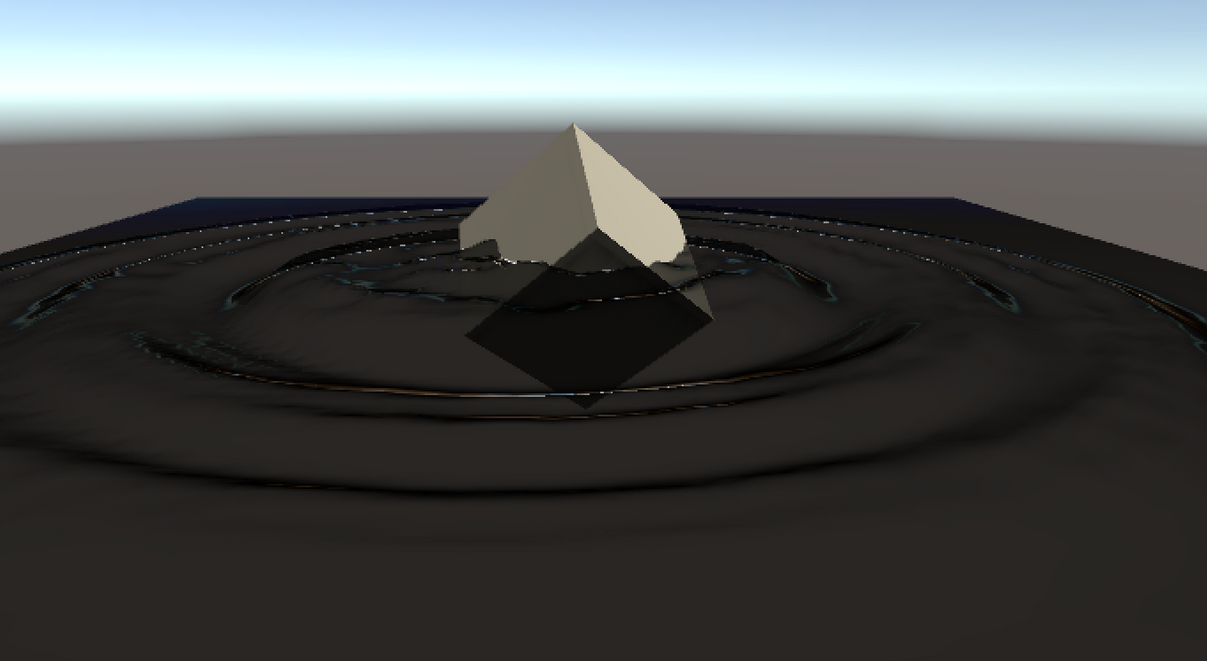
\includegraphics[width=0.8\linewidth]{waveparticles_example}
\caption{The modern 3D graphics card pipeline.}
\label{fig:waveparticles_example}
\end{figure}

There has been research into pushing forward the state-of-the-art in developing
code for heterogeneous platforms in more programmer-friendly ways. However, as
covered in Section \ref{sec:related_work}, much of the research has either been
domain-specific or provided abstractions which have an unacceptable performance
overhead for most use-cases involving GPUs. For example, a common approach is
to design a unified language which can be compiled to a run-time that supports
GPUs, as is the case with Lime \cite{Lime2010}. However, by hiding the details
of the heterogeneous backends the language targets, there is an unavoidable
run-time overhead. Working with current toolchains is an odd mix of using an
API and writing code in a GPU-specific language -- research has primarily
focused on hiding the API and simplifying GPU-specific elements by designing
unified languages abstract those details. However, alternative approaches which
improve aspects of current toolchains do exist.

The section provided the motivation for the solutions described in this paper,
first by demonstrating the prevalence of GPUs and how important improvements to
toolchains which target them could be. Secondly, it demonstrated the problems
current toolchains face with a brief example showing how data structures must be
defined separately in programming languages for the GPU and the CPU. Finally, a
brief explanation of why research has yet to tackle these problems was
provided.

\section{The Solutions}

This paper sections two solutions to the problems described above. First by
describing what the desired outcomes of those solutions should be and how they
should improve over the status quo. This is followed by what the solutions are;
first describing the annotation processor and then the pair of languages with a
unified type system. The pros and cons of each are then discussed to round off
the section.

\subsection{Desired Outcome}

As described in Section \ref{sec:related_work}, one of the largest stumbling
blocks that systems which aim to improve over current toolchains face is that
they sacrifice the control that traditional workflows provide in order to
improve the user-experience that programmers have. The issue with this approach
is the fact that performance is still important in many domains where GPUs are
used -- to the point where programmers still make the trade-off of working
directly with APIs like OpenGL instead of choosing the usability that
abstractions could otherwise provide. Therefore, solutions which aim to build
and improve upon the status quo should provide all the options that traditional
toolchains do, including exposing any underlying graphics APIs.

However, there are some ``easy wins'' to be made, as demonstrated by the
example shown in Listing \ref{lst:c_sharp_hlsl_struct_comparison}, which can be
found in compile-time type-checking. That is, instead of trying to unify code
that is written for the CPU and GPU under a single language or system, we can
acknowledge that they are different so have CPU code and shaders written in
different programming languages. This means that code written for the CPU
should still manually make API calls as it does in current toolchains. However,
this does not mean that shaders and CPU code should be entirely separate, and
we can still improve the programming model by having cross-language
type-checking to ensure we have achieve the level of consistency that is
desired.

Therefore, any solution that aims to improve upon current programming models
should give the benefits described above without sacrificing anything those
current systems provide.

\subsection{What was done}

I created two systems for type-checking programs accross language boundaries in
CPU-GPU systems. The first is a pre-processing system for C and GLSL that
operates on annotated sections of code. The second is a proof-of-concept pair
of languages with the features provided by the pre-processing system baked-into
the type system at the language level.

\subsubsection{Annotation System}

The annotation system reads annotated code written in C and annotated code
written in GLSL.


\subsubsection{New Language}

TODO:

\subsection{Pros and Cons}

TODO:


\section{Overview}

% This is the introduction where you should introduce your work.  In
% general the thing to aim for here is to describe a little bit of the
% context for your work -- why did you do it (motivation), what was the
% hoped-for outcome (aims) -- as well as trying to give a brief
% overview of what you actually did.

% It's often useful to bring forward some ``highlights'' into
% this chapter (e.g.\ some particularly compelling results, or
% a particularly interesting finding).

% It's also traditional to give an outline of the rest of the
% document, although without care this can appear formulaic
% and tedious. Your call.

TODO: Give overview of paper.

\section{Compelling Results}

TODO: Give compelling results.

\section{Summary}

TODO: summarise introduction.

\chapter{Technical Background}

\label{chp:technical_background}

% A more extensive coverage of what's required to understand your
% work. In general you should assume the reader has a good undergraduate
% degree in computer science, but is not necessarily an expert in
% the particular area you've been working on. Hence this chapter
% may need to summarize some ``text book'' material.

% This is not something you'd normally require in an academic paper,
% and it may not be appropriate for your particular circumstances.
% Indeed, in some cases it's possible to cover all of the ``background''
% material either in the introduction or at appropriate places in
% the rest of the dissertation.

% This chapter covers relevant (and typically, recent) research
% which you build upon (or improve upon). There are two complementary
% goals for this chapter:
% \begin{enumerate}
%   \item to show that you know and understand the state of the art; and
%   \item to put your work in context
% \end{enumerate}

% Ideally you can tackle both together by providing a critique of
% related work, and describing what is insufficient (and how you do
% better!)

% The related work chapter should usually come either near the front or
% near the back of the dissertation. The advantage of the former is that
% you get to build the argument for why your work is important before
% presenting your solution(s) in later chapters; the advantage of the
% latter is that don't have to forward reference to your solution too
% much. The correct choice will depend on what you're writing up, and
% your own personal preference.

This chapter provides extensive coverage of the relevant history of graphics
hardware and how it developed over time to become useful in many fields beyond
real-time rendering in video games. Following that, a breakdown of graphics
APIs is provided, to give both the context for the problem this paper aims to
tackle and the underlying technology the solutions depend upon. Then, the
difficulties and issues with programming for GPUs is summarised from the
contents of this chapter with a brief explanation of which ones the solutions
presented in this paper aim to tackle and which ones they do not. The chapter
finishes of with an overview of related research in this area, demonstrating
both were they succeed and how they fail to tackle the specific problems that
are solved here.

% TODO: Why low level details are important (eg unified memory versus seperate
% memory)
% https://www.slideshare.net/zlatan4177/gpgpu-algorithms-in-games
% https://en.wikipedia.org/wiki/Heterogeneous_System_Architecture

\section{GPU-CPU differences}



\begin{center}
\begin{tabular}{||c||c|c|c||}
\hline
        & Number of Cores  & FLOPS                                         & Type of parallelism \\
\hline
\hline
CPU     & 1 - O(10)        & Up to 1 Teraflop \cite{IntelTeraFlop}         & TODO                \\
\hline
GPU     & O(10) - O(10000) & Up to 100 Teraflops \cite{NVIDIA100TeraFlops} & TODO                \\
\hline
\end{tabular}
\end{center}

Can be worth being wary of GPU vs CPU performance based on perfomance alone.
http://people.eecs.berkeley.edu/~sangjin/2013/02/12/CPU-GPU-comparison.html



\section{A (brief) History of GPUs}

\label{sec:history_gpu}

Graphics Processing Units (GPUs) were originally fixed-function hardware
accelerators for 3D rendering aimed at hobbyist gamers who desired hardware to
play games with the most complex graphics possible \cite{TODO}. GPUs achieved
levels of fidelity that were otherwise unachievable by being focused on
optimising the \textit{rasterisation} step of 3D graphics rendering in
hardware. This allowed games using GPUs to display much higher levels of detail
(with higher framerates) compared to those using CPUs for rendering (known as
\textit{software rendering}). An early example of this was the video game Quake
and its update GLQuake. Whilst the former used the CPU for software rendering,
the latter supported GPUs through the use of the OpenGL API, allowing for
higher framerates, higher resolutions, improved texture filtering and
additional effects \cite{GLQuake}.

With time, developers wanted increasing artistic control over how video games
were rendered. Therefore, graphics cards stopped being fixed-function hardware
accelerators and the \textit{shader model} was created.

This gave graphics programmers some control over how computer graphics were
rendered. Although initially simple, as the desire for flexibility over these
systems increased, the capabilities of graphics cards themselves did so as
well, reaching a point where they are now essentially highly-parallel
general-purpose computation machines. A lot of the early (and current)
development of GPUs has been driven by a desire to increase the capabilities
they offer to video games, allowing them to drive not just traditional
rendering, but also physics \cite{TODO}, procedural world generation
\cite{TODO}, post-processing effects \cite{TODO} and alternative types of
rendering including ray-tracing \cite{TODO}.

\begin{figure}[h]
\centering

\includegraphics[width=0.8\linewidth]{TODO}
\caption{The modern 3D graphics card pipeline.}
\label{fig:graphics_pipeline}
\end{figure}

However, this increase in flexibility has allowed GPUs be used in increasingly
general domains, including scientific computing \cite{TODO}, crypto-currency
mining \cite{TODO}, video-processing \cite{TODO} and artificial intelligence
\cite{TODO}. To the point where the hobbyists the cards were originally
designed for are being priced out of the market \cite{TODO}.

\section{The Challenges with the APIs}

\label{sec:api_challanges}

\begin{table}
\footnotesize
\begin{tabu} to 1
\textwidth {||X[c]||X[c]|X[c]|X[c]||}
\hline
Name &
Created &
Developer &
Purpose \\
\hline
OpenGL &
1992 &
Khronos Group &
Graphics \\
\hline
Direct3D &
1996 &
Microsoft &
Graphics \\
\hline
CUDA &
2007 &
NVIDIA &
Compute \\
\hline
OpenCL &
2009 &
Khronos Group &
Compute \\
\hline
Metal &
2014 &
Apple &
Compute and Graphics \\
\hline
Vulkan &
2016 &
Khronos Group &
Compute and Graphics \\
\hline

\hline
\hline

\hline
Name &
Targets &
Langauge &
License \\
\hline
OpenGL &
GPUs &
GLSL and SPIR-V &
Open Specification \\
\hline
Direct3D &
GPUs with Windows OS &
HLSL &
Proprietary \\
\hline
CUDA &
NVIDIA GPUs &
CUDA C/C++ &
Proprietary \\
\hline
OpenCL &
GPUs, DSPs and FPGAs &
OpenCL C and SPIR-V &
Open Specification \\
\hline
Metal &
GPUs &
Metal Shading Language (C++ based) &
Proprietary \\
\hline
Vulkan &
GPUs (so far) &
SPIR-V &
Open Specification \\
\hline
\end{tabu}

\caption{ A comparison of different graphics and compute APIs, listed in
chronological order. }

\end{table}

This section gives an overview of the general challenges programmers face when
using graphics APIs. Firstly, the context and history of graphics APIs are
described, with a focus on OpenGL and Vulkan. Subsequently, the general
workflow of writing programs for GPUs is described, before finally the
individual problems that type heterogeneous type safety seeks to address are
identified.

Programmers interact with GPUs using APIs, however, as the development of and
growth of GPUs in computing has been relatively organic and ad-hoc, these APIs
themselves have many legacy components and can be difficult to work with.

To understand the challenges of working GPUs, one must first understand the
current workflow of GPUs and how that workflow has developed over time.

The best point of comparison is the CPU, and programming for the CPU. When
programming for the CPU, programmers often have access to a plethora of
programming languages which are suited to different needs and are capable of
targeting a wide range of backends. Furthermore, the instruction sets of CPUs
are published and well-documented, allowing programmers to write applications
for them directly -- even allowing them to write their own compiler for them
if they so desire. Finally, in the world of desktop computing, x86 is the
de-facto standard architecture, massively increasing the portability of
programs which target desktop PCs without the need for hardware abstractions
which could come with performance penalties.

The workflow of the GPU is very different.

\subsection{OpenGL}

Although GPUs do not have a standard ISA, open standards for GPU computing have
been developed and maintained by the Khronos Group \cite{TODO}, which was
founded in 2000 by a group companies for this purpose. OpenGL is the most
widely used standard graphics API that they maintain, however, the API has a
history dating back to the early 1990's \cite{TODO}, with control of the
standard being passed from Silicon Graphics in 2006 \cite{TODO}. For a long
time the OpenGL family of graphics APIs were the only cross-platform family of
graphics APIs, with OpenGL ES, a related API, being used for mobile and
embedded systems \cite{TODO}.

Despite OpenGL being an open standard with a differently-flavoured API for
non-desktop systems, portability and development using the API is difficult for
several reasons. The focus of this is on the language-aspects of graphics
programming.

The largest competitor to OpenGL has been Direct3D by Microsoft, and is an
alternative graphics API for Windows computers \cite{TODO}. Other platforms may
have their own proprietary graphics APIs, such a Metal for Apple devices
\cite{TODO}, and the various APIs that gaming consoles provide \cite{TODO}.
Although each of these platforms have their differences, the problems being
tackled can be generalised to all of them. Therefore, this paper will purely
focus on the OpenGL family of graphics APIs.

\subsection{Vulkan}

TODO:

\subsection{Graphics workflow and pipeline}

GPUs are highly parallel compute machines capable of running programs called
\textit{shaders}. However, unlike CPU programs, where a programmer will simply
start writing code in a \texttt{main} function which can be straightforwardly
compiled and executed, shaders require more setup and boilerplate. Typically,
shaders complement programs designed for the CPU, with the traditional example
being a video game. In this case, the core components of a game (such as logic,
animation, scene-setup, input handling) will be handled by the CPU which can
then offload certain computations to the GPU (such as graphics and physics).
The programmer does this by using graphics APIs to initialise the graphics
pipeline to the desired state for a particular computation (setting up buffers,
loading data onto the GPU, initialising the pipeline, reserving resources,
etc.). Following this, those APIs are used to direct the drivers to load
\textit{shader code} onto the GPU. Finally, the shaders are executed for the
desired results.

Although laborious, this workflow allows programmers to use the resources of
GPUs fairly efficiently. However, it is not without issues. The one which this
paper seeks to tackle is down to the fact that \textit{shaders} and CPU code
are written in completely different programming languages.

List to cover:

 - standard has a lot of legacy and issues:
    - different workflows and APIs for different applications
    - non-standard implementations of the standard, with vendor-specific extenions
    and other propietary technologies.
    - standard changes depending on whether targeting desktop, mobile or
    embedded systems
    - must interact with Operating systems directly, such as using their windowing
    system to create a \textit{context}. This reduces portabililty.
    - Langauges are compiled at run-time, with different shader-models
    - Companie wil partner with different vendors
    - Examples

\subsection{API options}

\label{sec:api_options}

TODO:


\textit{Issues Summary}

TODO;

\begin{lstfloat}
\begin{lstlisting}[language=C]
const float fixedDeltaTime;
const int currentFrame;
const float particleSpeed;
float2 getPosition(int startingFrame, float2 velocity, float2 origin) {
    float t = (fixedDeltaTime * (float)(currentFrame - startingFrame));
    return origin + (t * particleSpeed * velocity);
}

const int horiRes;
const int vertRes;
const float planeWidth;
const float planeHeight;
StructuredBuffer<WaveParticle> waveParticleBuffer;
RWTexture2D<float4> amplitudeTexture;

///
/// Splat the wave particles to the splatTexture
///
#pragma kernel SplatParticles
[numthreads(THREAD_GROUPS_X, 1, 1)]
void DrawParticles(uint3 id : SV_DispatchThreadID)
{
    WaveParticle particle = waveParticleBuffer[id.x];
    float2 waveParticlePosition = getPosition(
        particle.startingFrame, particle.velocity, particle.origin
    );
    int xPos = (int)round((waveParticlePosition.x / planeWidth) * horiRes);
    int yPos = (int)round((waveParticlePosition.y / planeHeight) * vertRes);
    amplitudeTexture[int2(xPos, yPos)] +=
        float4(0.0, particle.amplitude, 0.0, 0.0);
}
\end{lstlisting}
\label{lst:draw_particles}
\caption{An example of an HLSL computer shader that takes a particle stored in
in a buffer and copies its amplitude to a specific location on a texture.}
\end{lstfloat}

\section{Related Work}

\label{sec:related_work}

This section describes related work in the field of modifying or improving GPU
toolchains beyond traditional low-level libraries. It aims to show diverse set
of approaches that have been taken to doing this and the progress that has been
made, in addition to demonstrating the specific problems targeted by this paper
have yet to be addressed.

Since the creation of the SPIR-V intermediate language for heterogeneous
programming (as discussed in Chapter \ref{chp:technical_background}), some
progress has been made in simplifying and unifying how GPUs are interacted with
for compute purposes. In addition to a modified version of C, \textit{OpenCL
C}, OpenCL has recently standardised a modified version of C++, \textit{OpenCL
C++} for developing compute kernels \cite{OpenCL22Release}
\cite{OpenCLCPPWhitePaper} \cite{OpenCL}. However, despite unifying some
aspects of host and accelerator languages, this uses the traditional workflow
of programming compute kernels and host code separately, with no cross-module
checking at the API boundaries \cite{OpenCL22Release}. SYCL is a framework
built on top of OpenCL that abstracts away the API calls to enable
``single-source'' C++ development which automatically generates host and kernel
from a single C++ source file \cite{OpenCL22Release} \cite{SYCL}. SYCL has seen
uptake in terms of multiple implementations \cite{ComputeCPP} \cite{triSYCL},
and has been adopted as a backend for various machine learning frameworks such
as TensorFlow and Eigen \cite{SYCLTensorFlow} \cite{SYCLEigen}. However, this
approach does have its limitations in removing the ability for developers to
control how those API calls are made. Both OpenCL and SYCL are also limited in
only being suitable for \textit{compute} applications, and do not allow for the
graphics operations that GPUs are capable of. However, Vulkan and OpenCL could
merge in the future \cite{VulkanOpenCLMerge}.

Research has been done to make GPU and heterogeneous computing available in
high level languages. There are several approaches to this. The most
straight-forward is to abstract a compute platform such as OpenCL or CUDA using
a framework or library, which has primarily seen success in fields such as
scientific computing and machine learning. Theano and TensorFlow do this
\cite{Theano2016} \cite{TensorFlowWhitePaper}.

Harlan, developed by Holk et al, is a dommain-specific langauge based on Scheme
for GPUS, with support for higher order programming with Scheme-influenced
syntax and semantics \cite{Harlan} \cite{HarlanAnnouncement}. GPipe extends the
functional language Haskell such that shaders can be written functionally and
OpenGL calls can be made in type-safe ways, however, the garbage-collected
nature of Haskell makes it unsuitable for many of the domains GPUs are used
such as games \cite{HaskellState} \cite{GPipe}. Halide is another DSL for image
processing and comuptational photography \cite{Halide}.

Another approach has that has been taken is to abstract away underlying APIs
such as CUDA and OpenCL with platforms that can target both as backends. HIP is
a project that does this by allowing CUDA code to be compiled to C++ that uses
an abstracted API so that developers can convert their CUDA projects which is
NVIDIA's proprietary language that can only target NVIDIA GPU to something that
can target arbtrary backends \cite{HIP}. Lime and JCUDA take the approach of
compiling Java or Java-like for heterogeneous architectures \cite{Lime2010}
\cite{Lime2012} \cite{JCUDA2009}. However, they different in their approaches.
Lime aims to abstract low-level details of heterogeneous such that arbtrary
backends can be targetted, including GPUs (using OpenCL as a back-end) and FPGA
syncthesisation. JCUDA is much more specialised, specifically allowing CUDA
programs to be created using Java, with an interface that aims to closely match
CUDA's native C one so that code can target it specifically.

OpenACC is a system specifically targeted at scientists that lets programmers
mark appropriate sections of normal C++, C or Fortran code as possible
candidates for accelerated parallel computation \cite{OpenACC}. The goal is
specifically to allow users to write code as they normally would for the CPU,
and then perform a pass where that code is left entirely unmodified except for
the addition of directives.

Fumero et al. have developed techniques to automatically offload computation
from high-level interpreted dynamic languages using just-in-time compilation to
achieving speedups by compiling R to an OpenCL C backend \cite{JITGPU}.

Futhark is an attempt to design a functional data-parallel array language from
the ground-up that can target GPUs, targetting an OpenCL backend
\cite{Futhark}.

In addition to SYCL and OpenCL C++, there have been other attempts at bringing
heterogeneous programming models natively to C++ specifically through parallel
programming standards. C++ AMP is a C++ library, programming model, and
compiler developed by Microsoft that targets DirectX 11 \cite{CAMP}. However,
it seems to have died \cite{CAMPFail1} \cite{CAMPFail2}. \textit{C++ extensions
for parallelism} has brought such standards to the C++ standard template
library \cite{CPPParallelism}. Finally, OpenMP is an API standard dedicated to
shared-memory multiprocessing \cite{OpenMP}. HCC is a project aims to take C++
code that conforms to any of these standards and compile it to AMD's GCN
instruction set \cite{HCC}.

The biggest problem with all of these though is that they focus on abstracting
underlying API calls that are made to enable heterogeneous programming,
exposing alternate high-level interfaces to ensure simplified and less
error-prone program. This differs from the approach taken here, which is to
programmers to mark-up uses of those API calls directly so that they are
checked and compile-time for consistency without sacrificing the control that
would otherwise be lost.

\chapter{Usage}

This chapter describes how the systems can be used by programmers.

TODO:

\chapter{Design}

The heterogeneous type checking aspects of the projects is composed of two
alternative systems. The first is a pre-processing system for C and GLSL that
ensures the enforcement of interfaces between the two languages. The second is
a set of two novel toy languages which natively support such enforcement.

\section{Design Goals}

The ultimate design goal of the cross-module type checking systems is to make
programming for GPUs less frustrating and error prone by catching errors which
can commonly occur. However, unlike other systems which do this, we cannot have
\textit{any} compromises to runtime performance relative to existing industry
standards such as GLSL and OpenGL. This includes not limiting the possible
programs programmers can make. Naturally there pros and cons to this approach.

There are other concerns beyond performacne that need to be taken into account
which inform the design the system. For example, a commonly used feature is two
\textit{swap} shaders with identical interfaces in-and-out at runtime.
Therefore this needs to be supported by the system as well.

\begin{itemize}

    \item Having a non-intrusive system

    \item supporting simple workflows, but without sacrificing control

    \item Allow different shaders to be type-checked at compile-time but
    swapped in-and-out at run-time.

    \item Allow custom wrappers to exist.

\end{itemize}

\section{Workflow}

One of the important parts of the system is the implementation of the workflow.

\section{Annotation Processor}

TODO

\section{Language}

TODO

\chapter{Implementation}

% This chapter may be called something else\ldots but in general
% the idea is that you have one (or a few) ``meat'' chapters which
% describe the work you did in technical detail.

The source code for the project is publicly available and open-source
\cite{ProjectSource}. The implementation is formed of two distinct components,
the C-annotation pre-processor and the custom-languages compiler. Although both
are written in C++, Python is also used as a build-system to enable simple
cross-platform builds. The project was developed and tested on both Ubuntu
16.04 and Windows 10 operating systems.


\section{Pre-processor}

TODO:

\section{Compiler}

TODO: reference usage of FNV hash for symbol table. \cite{FNVHash}.


\chapter{Evaluation}

% For any practical projects, you should almost certainly have
% some kind of evaluation, and it's often useful to separate
% this out into its own chapter.


\section{Performance}

Ideally, there shouldn't be any performance overhead in either of the
solutions. For the annotation processor, that's fairly straight-forward to
establish, as it is essentially syntactic sugar that sits on-top-of C and GLSL.

However, although the custom language has semantics very similar to C and GLSL,
and in theory identical programs in both environments should be \textit{just
as} performant as C - the compiler may not optimise as well as it should.

TODO:


\chapter{Conclusion, Further Work and the Future of Heterogeneous Programming}

% As you might imagine: summarizes the dissertation, and draws
% any conclusions. Depending on the length of your work, and
% how well you write, you may not need a summary here.

% You will generally want to draw some conclusions, and point
% to potential future work. \cite{DirectXWorkings}

TODO:

\appendix
\singlespacing

\bibliographystyle{unsrt}
\bibliography{references}

\end{document}
